\documentclass{report}
\usepackage{graphicx}
\usepackage{pgfplots}
\begin{document}
\begin{titlepage}
\centering
{\bfseries\LARGE Instituto Tecnol\'ogico de Costa Rica \par}
\vspace{1cm}
{\scshape\Large Facultad de Ingenier\'ia en Computaci\'on \par}
\vspace{3cm}
{\scshape\Huge Falling Code\par}
\vspace{3cm}
{\itshape\Large Tarea 1\par}
\vfill
{\Large Fabrizio Alvarado Barquero\par}
{\Large 2017073935\par}
\vfill
{\Large Septiembre 2020 \par}
\end{titlepage}
\newpage
\section{Introduci\'on}
\newline
El problema a solucionar es la implementaci\'on de un sistema operativo llamado MacOS, el cual nos va a ayudar a comprender de una mejor manera el funcionamiento del booteo de una computadora, como funciona este proceso en si y como est\'a compuesto y estructurado en cuanto a los elementos de este proceso. \newline
\newline
El sistema MacOS presenta una unica funcionalidad, la cual es la animaci\'on de 'Falling Code' tal como la que se presenta en la pel\'icula The Matrix, donde el programa constantemente esta imprimiendo caracteres para no dejar de hacer la simulaci\'on de 'falling'. Adem\'as permite que el usuario ingrese caracteres deseados mediante el teclado y estos mismos son impresos con la animaci\'on previamente descrita.
\newpage
\section{Ambiente de desarrollo}
- QEMU: \newline Sistema emulador de software. \newline
\newline
- Geany: \newline Editor de texto. \newline
\newline
- GitHub: \newline Control de versiones. \newline
\newline
- Oracle Virtual Box: \newline Emulador para verificaci\'on del resultado final. \newline
\newline
\newpage
\section{Estructuras de datos usadas y funciones}
* Funciones \newline
\newline
- start: \newline
Funci\'on inicial del programa, esta activa el modo video, cambia el color de fondo y setea el cursor. \newline
\newline
- code: \newline
Funci\'on recursiva del programa, la cual revisa el input, en caso de haber algo dentro, llama a la funci\'on respectiva de imprimir, de no haber nada, llama al timer e imprime el caracter default y finalmente llama de nuevo a esta misma funcion para iniciar nuevamente el proceso. \newline
\newline
- printcharacterDefault: \newline
Imprime la secuencia de columnas a lo largo de la pantalla con caracteres default. \newline
\newline
- imprimirDefault: \newline
Imprime el caracter default utilizado, el cual es 1 ASCII (una carita fel\'iz). \newline
\newline
- printcharacter: \newline
Imprime la secuencia de columnas a lo largo de la pantalla con el caracter ingresado. \newline
\newline
- inputcharacter: \newline
Lee el caracter ingresado. \newline
\newline
- timer: \newline
Realiza un delay de aproximadamente 2 segundos entre caracteres. \newline
\newline
- scrollDown: \newline
Realiza la funci\'on de bajar el scroll de la pantalla 3 renglones. \newline
\newline
- imprimir: \newline
Imprime el caracter previamente ingresado. \newline
\newline
\newline
* Estructuras \newline
\newline
- No hay estructuras como tal, el programa es muy lineal. \newline

\newpage
\section{Instrucciones para ejecutar programa}
\newline
- Generaci\'on de .bin desde el .asm: \newline
nasm -f bin -o [elBinario].bin [elEnsamblador].asm\newline
\newline
- Emulaci\'on del sistema en plataforma QEMU: \newline
qemu-system-i386 -fda [elBinario].bin \newline
\newline
-Configuraci\'on y generaci\'on del .iso: \newline
nasm -f bin -o boot.bin boot.asm \newline
dd if=/dev/zero of=floppy.img bs=1024 count=1440\newline
dd if=boot.bin of=floppy.img seek=0 count=1 conv=notrunc\newline
mkdir iso\newline
cp floppy.img iso
genisoimage -quiet -V 'MYOS' -input-charset iso8859-1 -o myos.iso -b floppy.img \
    -hide floppy.img iso/
\newline
\newline
- Ejecutar el MacOS en VB: \newline
Crear una maquina virtual y seleccionar el .iso
\newpage
\section{Actividades realizadas por estudiante}
\newline
{\underline {Viernes 25 de septiembre - 5 horas}
\newline
-Instalación de herramientas como qemu y nasm \newline
-Investigación sobre booteo MBR\newline
-Se refresco el lenguaje ensamblador mediante un hello world\newline
-Investigacion e implementacion de ejemplo de lectura y escritura de usuario\newline
\newline
Problemas:No logre implementar ejemplo de lectura y escritura en el qemu, únicamente como programa corriente de assembly
\newline
\newline
{\underline {Sábado 26 de septiembre - 5 horas}}
\newline
-Investigué sobre cómo funciona realmente el booteo ya que estaba trabajando sobre un programa de ensamblador “normal”. \newline
-Tuve que iniciar un documento nuevo ya que los tenía no funcionaban de manera “booteable”\newline
-Logre implementar una lectura y escritura de letras, además del video mode y el color de las letras.\newline
-Termine el día de trabajo “traveseando” la funcionalidad de mover cursor para acomodar las letras que se van digitando.\newline
\newline
Problemas:
No logro encontrar una fórmula o algo por estilo para lograr el efecto de “falling”, además de otros detalles como ir eliminando los caracteres antiguos.
\newline
\newline
{\underline {Lunes 28 de septiembre - 3 horas}
\newline
-Pensé alguna manera de mejorar el efecto falling, pero no se me ocurre ninguna solución con notable mejora a la antigua. \newline
-Mejoré algunos detalles como el color de fondo del DOS y ocultar el cursor.\newline
-Investigue sobre la generación del ISO.\newline
-Documentación de código.\newline
-Documentación de tarea.\newline
\newline
Problemas:
No logre generar el iso correctamente.
\newline
\newline
{\underline {Martes 29 de septiembre - 6 horas}
\newline
-Se añade funcionalidad del efecto falling\newline
-Se añade funcionalidad de un timer\newline
-Se añade funcionalidad de que la pantalla haga scroll para abajo aun cuando el usuario no está digitando caracteres\newline
-Investigue más sobre la generación del .iso \newline
\newline
\newline
Problemas:
Me falta poder generar correctamente el iso
\newline
\newline
\newline
{\underline {Miércoles 30 de octubre - 3 horas:}
\newline
-Investigué aún más sobre booteo ya que ninguna de las anteriores me funcionó.\newline
-Logré encontrar una página de Stack Overflow donde me funcionó la generación del iso.\newline
-Logré bootear correctamente el iso generado en VirtualBox.\newline
-Finalizaci\'on de documentaci\'on\newline
\newline

\newpage
\section{Autoevaluaci\'on}
\newline
\newline
- Estado final: \newline
El estado final del programa MacOS es tal como se pidi\'o en la especificaci\'on, \newline
un sistema booteable que permite ver una animaci\'on de falling code.\newline

\newline
\newline

- Problemas:\newline
El unico problema existente es que no tiene el nivel de detalle que se ve\'ia en el 
video de ejemplo del programa en The Matrix, pero b\'asicamente y en esencia es igual. \newline

\newline
\newline

- Limitaciones:\newline
Creo que no hubo ninguna limitaci\'on mas all\'a de mi pobre conocimineto en el lenguaje utilizado.\newline
\newline

Evaluaci\'on: \newline

\begin{tabular}{x y z}
Caracter\'istica & Valor & Obtenido estimado \\ \hline
Arranque & 30 & 30\\
MacOS & 50 & 45\\
Documentaci\'on & 20 & 15\\
Extra & 10 & 0\\ \hline
Total & 110 & 90 \\ \hline
\end{tabular}
\newline
\newline
\newline
\newline
\begin{center}
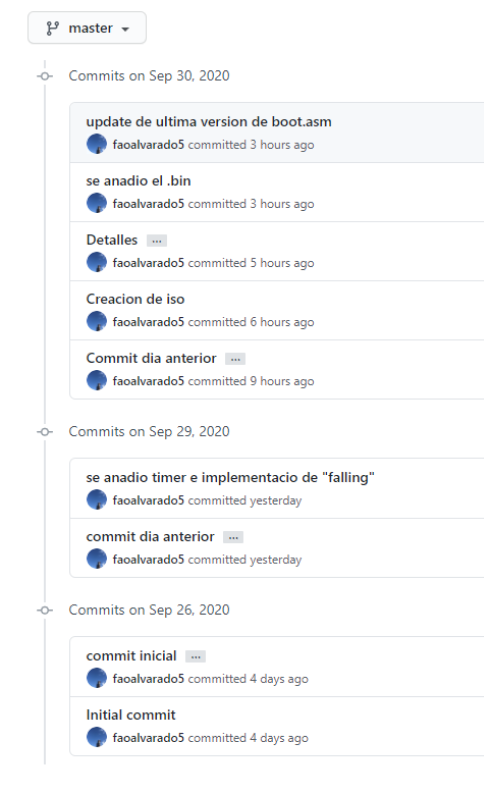
\includegraphics[scale=0.7]{Capture.png} 
\end{center}
\newline
\newline
-Repositorio de GitHub: \newline
https://github.com/faoalvarado5/tarea1Operativos \newline
\newline
-Reporte de commits: \newline
https://github.com/faoalvarado5/tarea1Operativos/commits?author=faoalvarado5

\newpage
\section{Lecciones aprendidas}

En lo personal me gust\'o mucho la tarea, ya que por m\'as dificil que fuera y 
dem\'as, refresqu\'e y reforc\'e mucho mi conocimiento sobre el lenguaje esamblador, debido a que
desdichadamente mi curso de Arquitectura no fue el mejor.\newline
\newline
\newline
M\'as puntualmente, aprend\'i el proceso de arranque de un sistema operativo y como este bootea desde que
se presiona el bot\'on de inicio de la computadora.\newline
\newline
\newline
Finalmente, pero no menos importante, aprend\'i a organizarme y trabajar de una manera adecuada bajo presi\'on, ya que en menos de una semana logr\'e aprender un lenguaje, una funcionalidad vital de la 
computadora como el arranque y como esta est\'a compuesta.

\newpage
\section{Bibliograf\'ia}

\newline
- Gabrielececchetti.it. (2020). Retrieved 1 October 2020, from \newline http://www.gabrielececchetti.it/Teaching/CalcolatoriElettronici/Docs/i8086_and_DOS_interrupts.pdf. \newline
\newline
- Assembly Language. Vitaly_filatov.tripod.com. (2020). Retrieved 1 October 2020, from \newline http://vitaly_filatov.tripod.com/ng/asm/.
\newline
\newline
- 2-main_menu - Tech Help!. Techhelpmanual.com. (2020). Retrieved 1 October 2020, from \newline http://www.techhelpmanual.com/2-main_menu.html.
\newline
\newline
- INT 10H. En.wikipedia.org. (2020). Retrieved 1 October 2020, from \newline
https://en.wikipedia.org/wiki/INT_10H.
\newline
\newline
- FLAGS register. En.wikipedia.org. (2020). Retrieved 1 October 2020, from \newline https://en.wikipedia.org/wiki/FLAGS_register.
\newline
\newline
- 16-bit computing. En.wikipedia.org. (2020). Retrieved 1 October 2020, from \newline https://en.wikipedia.org/wiki/16-bit_computing#:~:text=A%2016%2Dbit%20integer%20can,KB%20of%20byte%
\newline
\newline
- bootloader, C., Abdel-Rahman, M., & Petch, M. (2020). \newline
Creating a bootable ISO image with custom bootloader. Stack Overflow. Retrieved 1 October 2020, from \newline
https://stackoverflow.com/questions/34268518/creating-a-bootable-iso-image-with-custom-bootloader.
\newline

\end{document}